\documentclass[13pt]{article}
\renewcommand{\baselinestretch}{1.2}
\usepackage[utf8]{vietnam}
\usepackage[a4paper, total={6in, 8in}]{geometry}
\usepackage[vietnamese,english]{babel}
\usepackage{hyperref}
\usepackage{mathtools}
\usepackage{amssymb}
\usepackage{indentfirst}
\usepackage{graphicx}
\usepackage{minted}
\usepackage{ragged2e}
\usepackage{multirow}
\usepackage{subcaption}
\usepackage{xurl}
\usepackage{amsmath}
\usepackage{makecell}
\renewcommand\theadalign{bc}
\renewcommand\theadfont{\bfseries}
\renewcommand\theadgape{\Gape[4pt]}
\renewcommand\cellgape{\Gape[4pt]}
\usepackage{pbox}

\graphicspath{ {./graphics/} }

\hypersetup{
    colorlinks=true,
    linkcolor=blue,
    citecolor=blue,
    urlcolor=blue,
}

\usepackage[nottoc]{tocbibind}

\begin{document}
\begin{titlepage}
    \begin{center}
        \vspace*{1.8cm}
        \Large
        Distributed System Labwork 4\\
        \Large
        \vspace{0.5cm}
        \begin{center}
            
\includegraphics[scale=1.0]{images/usth_logo1.PNG}
        \end{center}  
        \vspace{0.5cm}
            Group 1 - ICT\\
        \vspace{0.5cm}
            University of Science and Technology of Hanoi\\
        \vspace{0.5cm}
            January, 2022
        \vfill
          
   \end{center}
\end{titlepage}

\newpage
\tableofcontents
\newpage


\section{Introduction}
\subsection{Overview}
\noindent%
Map-reduce is a programming model for distributed computing. It includes four main stages: splitting, mapping, shuffling, and reducing. Each stage is presented below:

\noindent%
- Splitting stage: Splitting is generally used during data processing in map-reduce programs. The input data is split equally based on user-defined. For example, a 100MB file can be split equally into four files; each file has a size of 25MB.

\noindent%
- Mapping stage: Each worker applies the map function to the data(usually in the file format). The mapper processes the data and creates several small chunks of data.

\noindent%
- Shuffling stage: Each worker nodes redistribute the data based on the output keys in a way such that all data with the same key belong to the same node

\noindent%
- Reducing stage: Each worker now processes the data after shuffling and produces the output


\subsection{Protocol}
\begin{figure}[h]
    \centering
    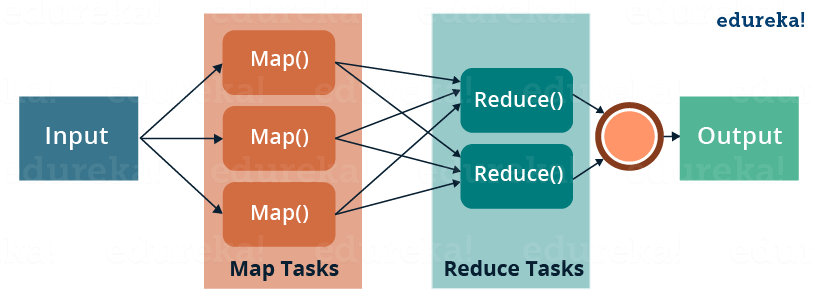
\includegraphics[scale=0.4]{images/mapreduce.png}
    \caption{Map-reduce process\cite{MPI word count}}
    \label{fig:protocol}
\end{figure}

\subsection{Framework}
\noindent%
We use C++ in this project, so we have to implement the map-reduce framework ourselves.

\section{Methodology}
\begin{itemize}
    \item We create one server and two slaves. First, we split the file in half and send the texts to each slave.
    \item Each slave will perform mapping and reducing.
    \item Afterwards, the server collects the slaver's results and prints out the results.
\end{itemize}

\section{Result}
\noindent%
This is a small part of the final result.
\begin{figure}[h]
    \centering
    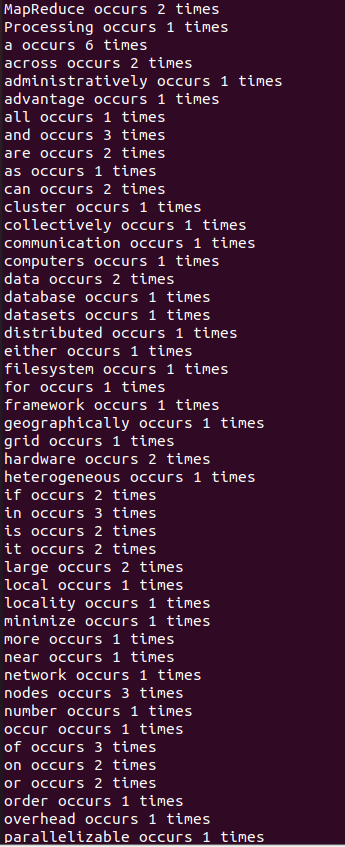
\includegraphics[scale=0.5]{images/result.PNG}
    \caption{Map-reduce program results}
    \label{fig:protocol}
\end{figure}

\begin{thebibliography}{9}
\bibitem{MPI word count}
https://www.oreilly.com/library/view/distributed-computing-in/9781787126992/5fef6ce5-20d7-4d7c-93eb-7e669d48c2b4.xhtml
\end{thebibliography}


\end{document}
